\documentclass[12pt]{article}
\usepackage[czech]{babel}
\usepackage[utf8]{inputenc}
\usepackage[plainpages=false,pdfpagelabels,unicode]{hyperref}
\usepackage[pdftex]{graphicx}
\usepackage[margin=2cm, includefoot]{geometry}

\begin{document}

\title{Experimentální metody a speciální praktikum \\
Volná povrchová energie}
\author{Vlasta Štěpánová, Roman Petráš a Pavel Ondračka}
\maketitle

\section{Úvod}
Voľnú povrchovú energiu látok môžeme definovať ako množstvo práce $W$ potrebnej na vytvorenie povrchu o jednotkovej ploche $\Delta A$. Rozmerovo aj číselne je rovná povrchovému napätiu $\gamma$. Platí 

\begin{equation}
W = \gamma \Delta A
\end{equation}
			
Voľnú povrchovú energiu je možné určiť metódou merania kontaktného uhlu usadenej kvapaliny na meranom povrchu.

Pri aplikácii tejto metódy je na očistený vodorovný povrch nanesené množstvo kvapiek testovacích kvapalín a meriame kontaktný uhol, uhol ktorý zviera dotyčnica k profilu kvapky v mieste styku troch fázy s rovinou povrchu pevnej látky. V rovnováhe je kontaktný uhol kvapaliny na povrchu pevnej látky určený mechanickou mechanickou rovnováhou systému kvapka – pevná látka – plyn, za pôsobenia troch druhou napätia s/l, s/v a l/v. na tvar povrchu kvapky má taktiež vplyv aj gravitácia, ktorý je možné eliminovať malými objemami testovacích kvapiek.

Stanovenie voľnej povrchovej energie pevnej látky meraním kontaktného uhla kvapaliny je založené na vzťahu rovnováhy troch medzifázových energii pomocou Youngovej rovnice

\begin{equation}
\gamma_\mathrm{sv} - \gamma_\mathrm{sl} = \gamma_\mathrm{lv} \cos{\theta}
\end{equation}

pričom $\gamma_\mathrm{sv}$ je voľná energia rozhrania s/v, $\gamma_\mathrm{sl}$ je voľná energia rozhrania s/l a $\gamma_\mathrm{lv}$  voľná energia rozhrania l/v, $\theta$ je kontaktný uhol.
Zmáčavosť kvapaliny na danom povrchu môžeme rozlíšiť. Pokiaľ je kontaktný uhol kvapaliny menší než pravý uhol, potom kvapalina povrch zmáča, naopak ak je kontaktný uhol väčší ako pravý uhol, kvapalina daný povrch nezmáča.

Ku stanoveniu celovej voľnej povrchovej energie môžeme postupovať dvoma prístupmi.

\begin{enumerate}
\item prístup\\
Využijeme stavovú rovnicu, vypočítame voľnú povrchovú energiu, kde celková energia závisí len na $\gamma_\mathrm{lv}$ a $\gamma_\mathrm{sv}$ vzťahom

\begin{equation}
\gamma_\mathrm{sl} = \mathrm{f}(\gamma_\mathrm{lv} , \gamma_\mathrm{sv}  )
\end{equation}

\item prístup\\
Využívame tzv. komponentové modely, ktoré sú založené na predpokladu, že voľná povrchová energia pevnej latky je mierou príťažlivých síl medzi povrchovou vrstvou pevnej látky s kvapalnou za predpokladu, že tieto príťažlivé sily a ich príspevky do celkovej energie sú aditívne. Medzimolekulárna príťažlivosť vyvolávajúca povrchové napätie pochádza zo známych medzimolekulárnych síl. 
\end{enumerate}



\section{Modely}
\subsection{Zismanov model}
Týmto modelom môžeme stanoviť hodnotu kritickej celkovej povrchovej energie $\gamma_\mathrm{c}$. Nameraním kontaktného uhla kvapky s viacerými kvapalinami a vynesením závislosti $\cos \theta = f (\gamma_\mathrm{l})$ dostávame Zismanov graf, ktorý má väčšinou lineárny priebeh. Extrapoláciou k nulovému kontaktnému uhlu $\cos 0^\circ = f (\gamma_\mathrm{c})$ dostaneme kritickú povrchovú energiu pevnej látky. Obvykle sa prekladá závislosť v tvare $\cos \theta = 1 + b (\gamma_\mathrm{c} - \gamma_\mathrm{l})$, pričom $b$ je konštanta charakteristická pre daný výber kvapalín. Model zanedbáva efekty ako napr. tlak šírenia a nie je schopný sledovať priebeh závislosti $\cos \theta = f (\gamma_\mathrm{l})$ pre veľké povrchové energie testovacích kvapalín. 

\subsection{Owens-Wendt-Rable-Kaeble model (OWRK)}
Celkovú povrchovú energiu môžeme určiť ako $\gamma = \gamma^\mathrm{d} + \gamma^\mathrm{p}$. Prvá zložka súčtu označuje prevažujúcu Londonovú disperznú interakciu a druhá – polárna zložka je tvorená prevažne interakciou vodíkových väzieb.

Za predpokladu Berthelotového kombinačného pravidla geometrických priemerov má model výsledný tvar
%
\begin{equation}
(1 + \cos \theta) \gamma_\mathrm{l} = 2 \left( \sqrt{\gamma^\mathrm{d}_\mathrm{s} \gamma^\mathrm{d}_\mathrm{l}} + \sqrt{\gamma^\mathrm{p}_\mathrm{s} \gamma^\mathrm{p}_\mathrm{l}}  \right) \, \mathrm{.} \label{owkr1}
\end{equation}
%
Ku stanoveniu dvojice komponent povrchovej energie je potrebné meranie kontaktného uhla s dvojicou kvapalín.

\subsubsection{Regresný model OWRK}
Rovnicu (\ref{owkr1}) upravíme do tvaru
%
\begin{equation}
\frac{1 + \cos \theta}{2} \frac{\gamma_\mathrm{l_i}}{\sqrt{\gamma^\mathrm{d}_\mathrm{l_i}}}
=
\sqrt{\gamma^\mathrm{d}_\mathrm{s}}
+
\sqrt{\gamma^\mathrm{p}_\mathrm{s}}
\sqrt{\frac{\gamma^\mathrm{p}_\mathrm{l_i} } {\gamma^\mathrm{d}_\mathrm{l_i} } } \, \mathrm{.} \label{owkr2}
\end{equation}
%
Uvedený zápis nám situáciu podstatne zjednoduší, keď ho budeme chápať ako rovnicu obecnej priamky $y = \beta_0 + \beta_1 x$.
Fitovaným rovnice (\ref{owkr2}) s rôznymi kvapalinami dostaneme výsledky pre komponenty $\gamma^\mathrm{d}_\mathrm{s}$ a $\gamma^\mathrm{p}_\mathrm{s}$.


\subsection{Acidobazický model}
Teória predpokladá, obdobne ako pri modely OWRK, že voľná povrchová energia ma dvojicu komponent $\gamma^\mathrm{TOT} = \gamma^\mathrm{LW} + \gamma^\mathrm{AB}$, pričom $\gamma^\mathrm{LW}$ je nepolárna Lifshitz-Van der Waalsová zložka, ktorá zahrňuje všetky van der Waalsové sily a $\gamma^\mathrm{AB}$ je polárna acidobazická zložka, ktorá je najčastejšie tvorená interakciou vodíkových väzieb spolu s kovalentnými väzbami.
$\gamma^\mathrm{AB}$ môžeme vyjadriť pomocou acidickej $\gamma^+$ a bazickej zložky $\gamma^-$ ako $\gamma^\mathrm{AB} = 2 \sqrt{\gamma^+ \gamma^-}$.

Povrchovú energiu môžeme psočítať pomocou Young-Drupého rovnice (\ref{acido1}). Dosadeným disperzných $\gamma^\mathrm{LW}$, kyslých $\gamma^+$ a zásaditých zložiek $\gamma^-$ kvapaliny a kontaktných uhlov daných kvapalín dostaneme sústavu troch rovníc pre trojicu neznámych parametrov testovaného povrchu (označené indexom $j$):
%
\begin{equation}
(1 + \cos \theta) \gamma_\mathrm{l} = 
2 \left(
\sqrt{\gamma^\mathrm{LW}_i \gamma^\mathrm{LW}_j }
\sqrt{\gamma^+_i \gamma^-_j }
\sqrt{\gamma^-_i \gamma^+_j }
\right) \, \mathrm{,} \label{acido1}
\end{equation}
%
kde index $i$ (ďalej už l) označuje kvapalinu a index $j$ (ďalej už s) pevnú látku – substrát. Hodnoty $\gamma^+_\mathrm{l}$, $\gamma_\mathrm{l}^-$ a $\gamma_\mathrm{l}^\mathrm{LW}$ sú známe a hodnoty $\gamma^+_\mathrm{s}$, $\gamma_\mathrm{s}^-$ a $\gamma_\mathrm{s}^\mathrm{LW}$ môžeme získať z merania kontaktného uhla s tromi kvapalinami.

Pokiaľ k popisu kvapalín používame väčšie množstvo kvapalín, bude sústava rovníc preurčená a pre výpočet $\gamma^+_\mathrm{s}$, $\gamma_\mathrm{s}^-$ a $\gamma_\mathrm{s}^\mathrm{LW}$ použijeme rovnicu (\ref{acido2}) a metódu najmenších štvorcov.
%
\begin{equation}
\frac{1 + \cos \theta}{2}
\frac{ \gamma_\mathrm{l}}{\sqrt{\gamma_\mathrm{l}^\mathrm{LW}}} = 
\sqrt{\gamma_\mathrm{s}^\mathrm{LW}} +
\sqrt{\gamma_\mathrm{s}^+}\sqrt{\frac{\gamma_\mathrm{l}^-}{\gamma_\mathrm{l}^\mathrm{LW}}}
\sqrt{\gamma_\mathrm{s}^-}\sqrt{\frac{\gamma_\mathrm{l}^+}{\gamma_\mathrm{l}^\mathrm{LW}}}
 \label{acido2}
\end{equation}
%
Pri porovnaní s metódou troch kvapalín, pri ktorej je možné použiť iba niektorých vhodných kombinácii kvapalín, je regresná metóda podstatne stabilnejšia.

\section{Měření}
Byly měřeny smáčivé úhly pro 5 kapalin: vodu, glycerol, ethylen-glykol, dijidometan a $\alpha$-bromnaftalen, měření jednotlivých kontaktních úhlů je uvedeno v tabulce \ref{uhly}. Průměrné vypočítané kontaktní úhly jsou v tabulce \ref{uhly-final}. Při vyhodnocování dat byly požity tři výše zmíněné modely: acidobazický, Zismanův a Owen-Wendtův. Všechny výpočty byly provedeny v programu See Software verze 6.3.

\subsection{Acidobazický model}
\begin{centering}
    $\gamma_\mathrm{total}$      =            54.38 $\pm$ 12.92 [mJ/m$^2$] (68.3\%)\\
    $\gamma_\mathrm{LW}$         =         33.58 $\pm$ 6.19 [mJ/m$^2$] (68.3\%)\\
    $\gamma_\mathrm{AB}$         =           20.80 $\pm$ 11.35 [mJ/m$^2$] (68.3\%)\\
    $\gamma_\mathrm{+}$          =           2.54 $\pm$ 2.62  [mJ/m$^2$] (68.3\%)\\
    $\gamma_\mathrm{-}$          =           42.55 $\pm$ 15.26 [mJ/m$^2$] (68.3\%)\\
\end{centering}

\subsection{Owens-Wendtův model}
\begin{centering}
   $\gamma_\mathrm{total}$      =            60.90 $\pm$ 10.77 [mJ/m$^2$] (68.3\%)\\
    $\gamma_\mathrm{LW}$         =         31.00 $\pm$ 7.19 [mJ/m$^2$] (68.3\%)\\
    $\gamma_\mathrm{AB}$         =           29.90 $\pm$ 8.02 [mJ/m$^2$] (68.3\%)\\
    correl     =              0.98\\
\end{centering}

\subsection{Zismanův model}
\begin{centering}
   $\gamma_\mathrm{total}$      =            101.28 $\pm$ 252.38 [mJ/m$^2$] (68.3\%)\\
    $b$         =         0.00 $\pm$ 0.01 (68.3\%)\\
    correl     =              0.30\\
\end{centering}


\begin{table}[htbp]
\begin{center}
\begin{tabular}{|c|c|c|c|c|c|}
\hline
\multicolumn{1}{|l|}{} & \multicolumn{5}{|c|}{Kontaktní úhel [$^\circ$]}  \\ \hline
Měření & Voda & Glycerol & Ethylene glycol & Diiodomethane & $\alpha$-bromonaphthalene \\ \hline \hline
1 & 28,377 & 23,001 & 7,976 & 49,045 & 31,598 \\ \hline
2 & 28,6 & 21,506 & 7,028 & 52,461 & 37,519 \\ \hline
3 & 28,6 & 23,039 & 6,297 & 53,294 & 45,985 \\ \hline
4 & 25,989 & 23,06 & 7,729 & 53,231 & 42,971 \\ \hline
5 & 26,977 & 22,738 & 9,064 & 52,665 & 39,516 \\ \hline
6 & 29,443 & 23,827 & 9,031 & 48,711 & 44,576 \\ \hline
7 & 32,582 & 21,416 & 9,468 & 51,091 & 41,071 \\ \hline
8 & 31,599 & 22,72 &  & 49,251 &  \\ \hline
9 & 31,411 &  &  &  &  \\ \hline
10 & 26,16 &  &  &  &  \\ \hline
11 & 28,456 &  &  &  &  \\ \hline
\end{tabular}
\caption{Naměřené kontaktní úhly pro jednotlivé kapaliny, počet měření pro jednotlivé kapaliny není stejný kvůli vyřazení vybočujících hodnot}
\label{uhly}
\end{center}
\end{table}

\begin{table}[htbp]
\begin{center}
\begin{tabular}{|l|c|}
	\hline
     Kapalina & Kontaktní úhel [$^\circ$] \\ \hline \hline
    Voda                   &  28.93 $\pm$ 2.64 (99.9\%) \\ \hline
    Diiodomethane          &  51.22 $\pm$ 3.18 (99.9\%) \\ \hline
    Glycerol               &  22.66 $\pm$ 1.33 (99.9\%) \\ \hline
    Ethylene glycol        &  8.08  $\pm$ 2.20 (99.9\%) \\ \hline
    $\alpha$-bromonaphthalene     &  40.46 $\pm$ 9.17 (99.9\%) \\ \hline
\end{tabular}
\caption{Výsledné kontaktní úhly pro různé kapaliny}
\label{uhly-final}
\end{center}
\end{table}


\begin{figure}[ht]
\begin{minipage}[b]{0.5\linewidth}
\centering
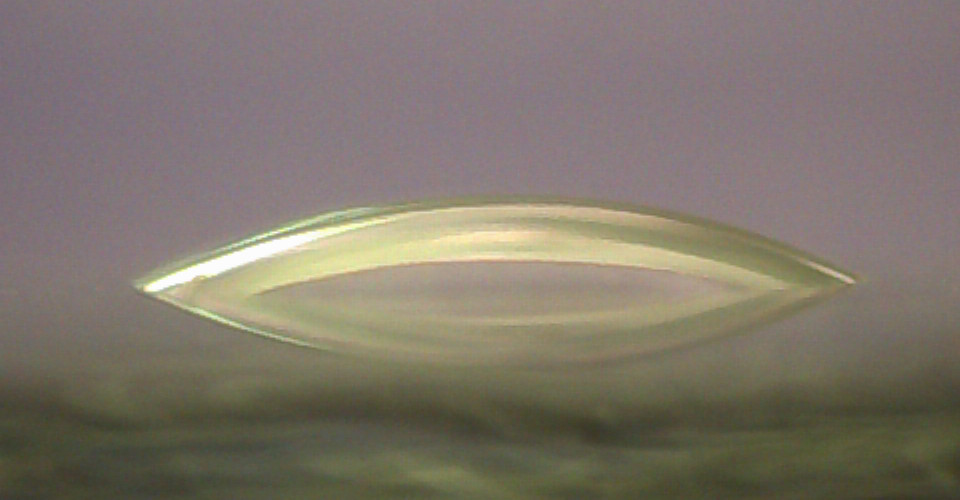
\includegraphics[width=200px]{img/w.jpeg}
\caption{Voda}
\label{fig:water}
\end{minipage}
\begin{minipage}[b]{0.5\linewidth}
\centering
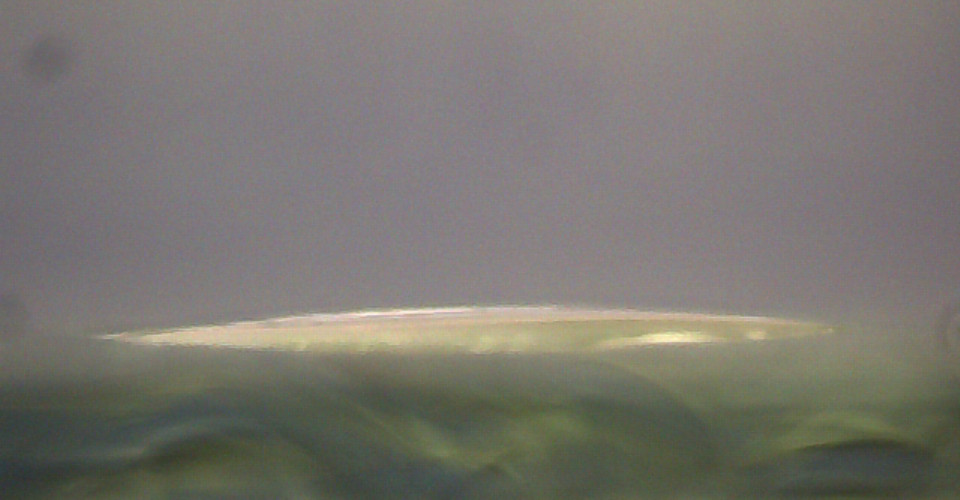
\includegraphics[width=200px]{img/eg.jpeg}
\caption{Ethylene glycol}
\label{fig:eg}
\end{minipage}

\hspace{1.5cm}

\begin{minipage}[b]{0.5\linewidth}
\centering
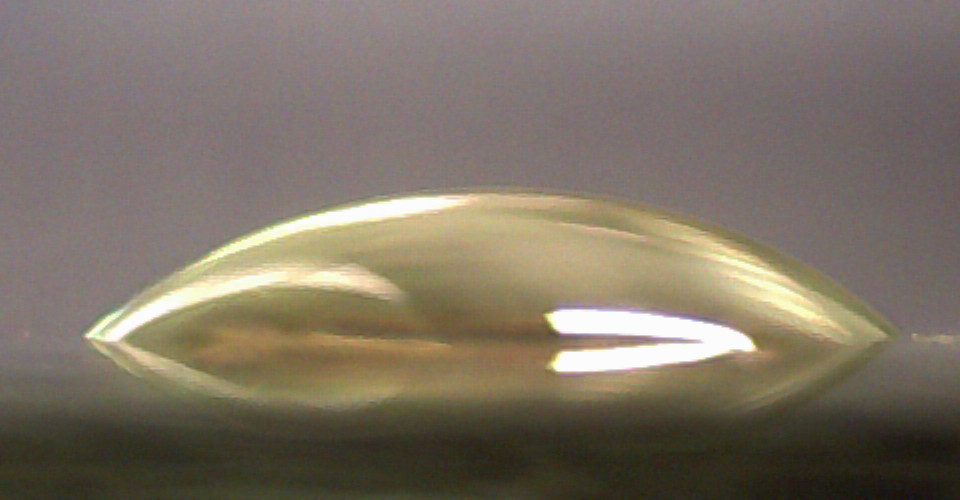
\includegraphics[width=200px]{img/ab.jpeg}
\caption{$\alpha$-bromonaphthalene}
\label{fig:ab}
\end{minipage}
\begin{minipage}[b]{0.5\linewidth}
\centering
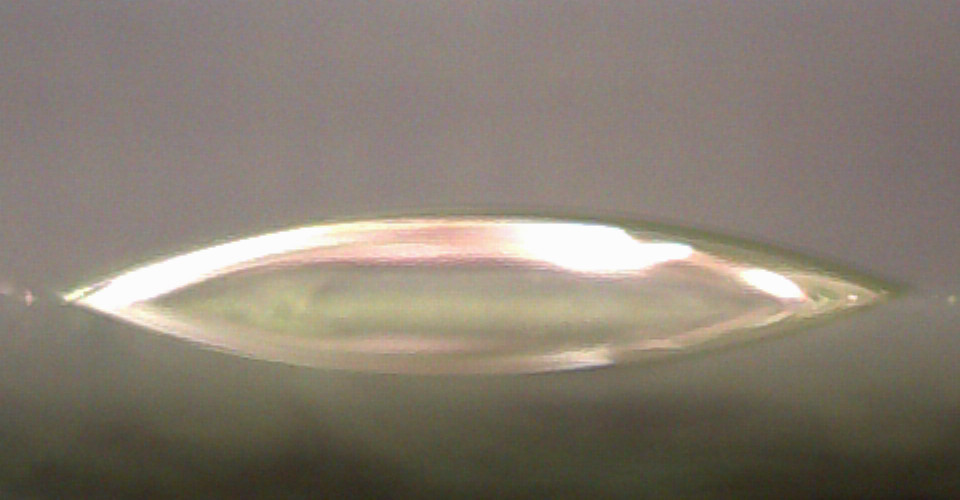
\includegraphics[width=200px]{img/g.jpeg}
\caption{Glycerol}
\label{fig:g}
\end{minipage}

\hspace{1.5cm}

\begin{minipage}[b]{1\linewidth}
\centering
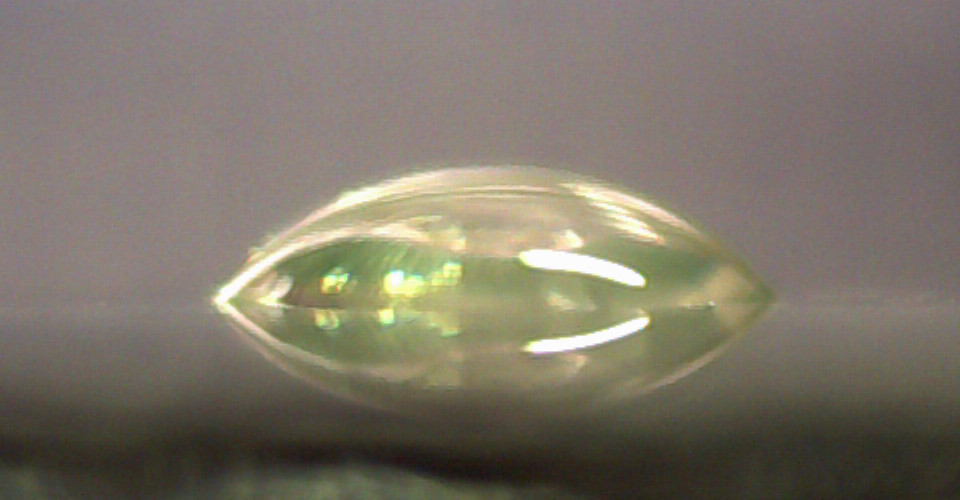
\includegraphics[width=200px]{img/d.jpeg}
\caption{Diiodomethane}
\label{fig:d}
\end{minipage}
\end{figure}

\newpage
\section{Závěr}
Měření proběhlo úspěšně. Na přístroji SEE System se nám podařilo naměřit kontaktní úhly pěti měřených kapalin na substrátu. Velký rozptyl naměřených úhlů pro jednotlivé kapaliny byl způsoben pravděpodobně malou zručností při pipetování a odečítání z obrázků, z těchto chyb poté bohužel vyplývá i velká nejistota ve výsledcích. Co se týče výsledků, acidobazický model i Owens-Wendtův model dávají podobné výsledky s celkovou energií 54.38 $\pm$ 12.92 [mJ/m$^2$] a 60.90 $\pm$ 10.77 [mJ/m$^2$], také Lifshitz-Van der Waalsovy a acidobazické složky vycházejí podobně. Zismanův model bohužel dává odlišné výsledky, tyto jsou nicméně zatíženy velmi velkou chybou.

\end{document}
